\chapter{Aplikacja rozwiązująca problem przydziału kwadratowego z wykorzystaniem kwantowego algorytmu ewolucyjnego}
\label{cha:aplikacja}
Jednym z celów realizowanej pracy dyplomowej było napisanie aplikacji, która przy wykorzystaniu jednego z algorytmów aproksymacyjnych będzie rozwiązywać problem przydziału kwadratowego. Wybór padł na kwantowy algorytm ewolucyjny NPQGA opisany w rozdziale czwartym. Uwzględnione w nim zmiany oraz modyfikacje zostały przedstawione w piątym rozdziale. Program został zrealizowany jako aplikacja konsolowa i napisana w języku C\#. O tym, że aplikacja będzie konsolowa zadecydował fakt, iż jej celem nadrzędnym jest znajdywanie rozwiązania problemu QAP i ma służyć jako narzędzie pozwalające zweryfikować działanie algorytmu. Aspekty wizualne są jedynie dodatkiem, który nie wpływa na jakość rozwiązania problemu.

\section{Interfejsy klas}
Punktem wyjścia do rozpoczęcia prac był zestaw interfejsów klas przygotowanych przez opiekuna niniejszej pracy. Interfejs klasy w sensie języka C\# jest narzędziem wykorzystywanym w technice dziedziczenia i określa metody i właściwości jakie klasa dziedzicząca po nim musi implementować. Jednakże ciała metod nie są określone i zależą wyłącznie od implementacji w danej klasie. W przeciwieństwie do dziedziczeniu po klasach, istnieje możliwość dziedziczenia po wielu interfejsach. Dzięki wykorzystaniu interfejsów, napisane na potrzeby pracy klasy będzie można wykorzystać w innych aplikacjach, czy to już istniejących, ale i w tych, które dopiero powstaną. Poniżej znajduje się lista interfejsów, które należało zaimplementować:
\begin{enumerate}
\item IEvolutionAlgorithm,
\item IOptimisationAlgorithm,
\item IPopulation,
\item ISolution,
\item IEvolutionaryOperator,
\item IMutationOperator,
\item ICrossoverOperator.
\end{enumerate}

Interfejs \textit{IEvolutionAlgorithm} dziedziczy po interfejsie \textit{IOptimisationAlgorithm}. Na bazie tych interfejsów powstała klasa \textit{QgAlgorithm} zawierająca metody pozwalające na ustawienie i uruchomienie algorytmu oraz pozwalająca na zwrócenie rezultatów działania algorytmu.

Interfejsy \textit{ICrossoverOperator} i \textit{IMutationOperator} dziedziczące po interfejsie \textit{IEvolutionaryOperator} posłużyły jako podstawa, dla stworzenia klas realizujących zadania operatorów krzyżowania oraz mutacji. Na podstawie interfejsu \textit{ICrossoverOperator} powstała również klasa reprezentują caoperator bramki kwantowej.

Interfejsy \textit{IPopulation} i \textit{ISolution} posłużyły do napisania klas reprezentujących odpowiednio pojedyncze rozwiązanie algorytmu i populację algorytmu.

\section{Struktura danych}
By algorytm mógł znaleźć rozwiązanie problemu, musi przetwarzać całą populację rozwiązań. Dlatego też została napisana klasa \textit{Population}, dziedzicząca po interfejsie \textit{IPopulation}. Populacja natomiast zawiera w sobie listę osobników, rozwiązań, które reprezentowane są przez obiekty klasy \textit{Solution} dziedziczącej z kolei po interfejsie \textit{ISolution}. Postacią rozwiązania w problemie przydziału kwadratowego jest permutacja, określająca, który obiekt został przypisany do kolejnych lokalizacji. Z tego powodu obiekty klasy \textit{Solution} zawierają w sobie listę obiektów reprezentujących elementy permutacji. Klasa tych obiektów została nazwana \textit{Chromosome}. Należy tutaj wyjaśnić pewną nieścisłość w terminach używanych w algorytmach genetycznych. \textit{Chromosomami} zwykło się nazywać kompletne rozwiązania, a ich fragmenty kodujące rozwiązanie \textit{genami}. Z racji, iż w aplikacji rozwiązania problemu reprezentowane są przez obiekty klasy \textit{Solution}, a element permutacji nie jest najmniejsza porcją informacji, postanowiono nazwać te porcje chromosomami, a ich najmniejszą część \textit{genem}. A więc \textit{chromosomy} składają się z kubitów reprezentowanych przez klasę \textit{Qbit}. Poprzez zdekodowanie stanu kubitów określa się wartość chromosomu, a następnie poprzez omówioną w rozdziale czwartym konwersję otrzymuje się permutacyjną postać rozwiązania problemu QAP.
\newpage
\begin{figure}[!t]
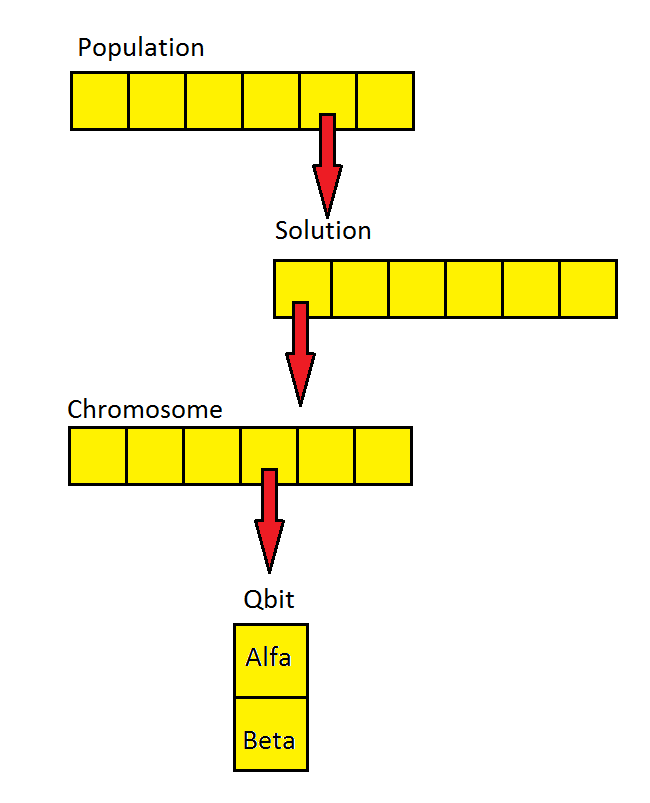
\includegraphics[scale=0.4]{data_structure}
\caption{Struktura danych}
\end{figure}

W kontekście struktury danych należy jeszcze wspomnieć o macierzach przepływu i odległości problemu QAP. Ich wartości są wczytywane z plików \textit{.dat} zawierających rozmiar problemu oraz odpowiednio macierze odległości i przepływu i są następnie trzymane w obiekcie klasy \textit{QapData} zrealizowanej jako singleton, czyli jako specjalna klasa o globalnym dostępnie pozwalająca na utworzenie tylko jednego jej obiektu. Posiada ona także mechanizmy, które bez wiedzy użytkownika same dbają o to, by faktycznie istniał jeden jej obiekt i jej instancja została utworzona podczas pierwszej próby jej użycia.

\section{Interfejs użytkownika}
Po uruchomieniu aplikacji użytkownik ma możliwość ustawienia kilku parametrów algorytmu. Należą do nich:
\begin{itemize}
\item wybór instancji problemu QAP,
\item rozmiar populacji, czyli ilość rozwiązań w populacji,
\item ilość iteracji algorytmu,
\item wybór sposobu selekcji rozwiązań,
\item wartość parametru $\eta_{max}$ w przypadku selekcji rankingowej,
\item minimalne i maksymalne prawdopodobieństwo krzyżowania,
\item operator krzyżowania,
\item prawdopodobieństwo mutacji,
\item wybór, czy stosować bramkę kwantową,
\item wersja bramki kwantowej,
\item wybór, czy otrzymane w wyniku działania algorytmu rezultaty i ustawione wartości parametrów zapisać do pliku,
\item nazwa pliku, do którego zostaną zapisane powyższe informacje.
\end{itemize}

W przypadku operatora selekcji do wyboru są dwie metody: ruletkowa oraz rankingowa. Spośród metod krzyżowania dostępne są trzy opcje: CX, OX i PMX. Wersje bramki kwantowej zostały opisane w rozdziałach 4 i 5.

Po zakończeniu zwracane są rezultaty działania algorytmu i możliwy jest ponowne uruchomienie algorytmu. Użytkownik ma możliwość wyboru spośród trzech opcji:
\begin{enumerate}
\item ponowne uruchomienie dla tych samych parametrów i tej samej populacji początkowej,
\item ponowne uruchomienie dla tej samej populacji, lecz dla nowych wartości parametrów, z oczywistym pominięciem ustawiania rozmiaru populacji a także wyboru instancji testowej,
\item wygenerowanie nowej populacji i ustawienie nowych wartości parametrów.
\end{enumerate}

Opcja pierwsza pozwala sprawdzić różnice w otrzymanych rezultatach działania algorytmu przy tych samych parametrach. W tej sytuacji można sprawdzić jaki wpływ na efekty końcowe ma czynnik losowy algorytmu.

Druga opcja pozwala na porównanie wpływu różnych wartości konkretnych parametrów na uzyskiwane rezultaty.

Opcja trzecia po prostu pozwala na ponowne uruchomienie algorytmu.

\section{Rezultaty działania aplikacji}
Po wykonaniu wszystkich iteracji algorytmu, program zwraca najlepsze znalezione rozwiązanie wraz z wartością funkcji celu oraz informację o tym, w której iteracji zostało zwrócone rozwiązanie. Zwracane jest również najlepsze rozwiązanie wraz jego wartością funkcji celu uzyskane w ostatniej iteracji algorytmu.

Jeśli została wybrana opcja zapisu do pliku, zapisane w nim zostają ustawione parametry algorytmu wraz z datą uruchomienia algorytmu, a także wartość najlepszego rozwiązania w każdej iteracji z informacją o średniej wartości rozwiązań w tej iteracji. W pliku zostaje też zawarta informacja o wartości najlepszego rozwiązania w ogóle wraz z numerem iteracji, w której zostało znalezione, a także jego postać. Podobnie, zawarta jest również informacja o najlepszym rozwiązaniu znalezionym w ostatniej iteracji. Zapis danych w formacie: nr iteracji, wartość średnia, wartość najlepszego rozwiązania w populacji pozwala potem na łatwy import danych do innych aplikacji pozwalających np. na utworzenie wykresów.

\section{Szczegóły związane z implementacją poszczególnych elementów algorytmu}
Kilka szczegółów związanych z działaniem algorytmu nie zostało poruszonych w publikacji[ref]. jednakże , by algorytm mógł działać, należało arbitralnie przyjąć pewne założenia. Jednym z takich założeń jest moment aktualizacji stanu kubitów. Zostało przyjęte w aplikacji, że należy ocenić w którym ze stanów 1 lub 0 znajduje się bit kwantowy, gdy aktualnie jego stan jest ustawiony na wartość -1. Wartość ta jest ustawiana w momencie, gdy zmienił się któryś z parametrów $\alpha$ i $\beta$ lub dopiero został utworzony obiekt klasy \textit{QBit}. Zmiana parametrów następuje zaś, gdy został spełniony warunek na zajście mutacji bądź kubit został poddany działaniu operatora bramki kwantowej. Zostało także przyjęte założenie, że efektem działania operatorów krzyżowania jest kombinacja dwóch rozwiązań z zachowaniem stanów kodujących ich kubitów. Wynika to z faktu, że operacje krzyżowania przeprowadzana jest dla wybranych na podstawie operacji selekcji rozwiązań w oparciu o ich funkcję celu, której wartość wynika z postaci tych rozwiązań i ocena stanów kubitów rozwiązań po krzyżowaniu powodowałaby, że otrzymane rozwiązania mogłyby nie mieć nic wspólnego z rozwiązaniami rodzicami.

W przypadku, gdy użytkownik programu postanowi, że algorytm ma znajdywać rozwiązanie bez wykorzystania bramki kwantowej, kwantowa idea algorytmu przejawia się wtedy jedynie podczas tworzenia populacji początkowej oraz operacji mutacji, która dalej polega na zamianie wartości parametrów $\alpha$ i $\beta$.

Rozwiązanie, które jest podstawą do działania bramki kwantowej i nazywane jest najlepszym, jest faktycznie najlepszym rozwiązaniem, ale uzyskanym w poprzedniej iteracji. Operator bramki kwantowej używany jest dopiero na populacji poddanej już działaniu operatorów krzyżowania i mutacji. Z tego powodu istnieje możliwość, że dopasowanie zapamiętanego rozwiązania będzie gorsze niż dopasowanie niektórych rozwiązań poddawanych działaniu bramki kwantowej. Dlatego rozważane są w tablicach \textit{Look Up} przypadki dla których warunek $f(x)>f(best)$ może być prawdą.